\begin{frame}{Equipe enseignante}
  \begin{columns}
    \begin{column}[T]{0.5\textwidth}
      \begin{itemize}
        \item Brest : \textbf{Jean-Christophe Le Lann}
        \begin{itemize}
          \item Enseignant-chercheur (Pr)
          \begin{itemize}
            \item ENSTA depuis 2009.
            \item Laboratoire LabSTICC UMR CNRS.
          \end{itemize}
          \item Ingénieur chez Thomson R\& D France
          \begin{itemize}
            \item 1999-2009 : conception des SoC de compression
          \end{itemize}
          \item Créateur et directeur technique startup
          \begin{itemize}
            \item Outils de CAO pour le codesign HW/SW.
          \end{itemize}
          \item Parcours :
          \begin{itemize}
            \item Habilitation à Diriger des Recherches.
            \item Thèse de doctorat d'Informatique.
            \item DEA de Microélectronique.
            \item Maîtrise de Physique fondamentale.
          \end{itemize}
        \end{itemize}
      \end{itemize}
    \end{column}
    \begin{column}[T]{0.5\textwidth}
      \begin{itemize}
        \item Référent Palaiseau : Pr. Omar Hammami
        \item Environ 12 intervenants
        \begin{itemize}
          \item Enseignant-cherheurs ENSTA
          \item Ingénieurs CEA
          \item Ingénieurs IN2P3
          \item Doctorants etc.
        \end{itemize}
      \end{itemize}
    \end{column}
  \end{columns}

  \begin{alertblock}{Remerciements}
    Support audio-visuel et pédagogique Brest-Palaiseau.
  \end{alertblock}
\end{frame}

\begin{frame}{Exemples de circuits et systèmes : broadcast vidéo}
  \begin{alertblock}{Société "Numérique"}
    \begin{itemize}
      \item usages, stockage...
      \item ...algorithmes et circuits complexes
    \end{itemize}
  \end{alertblock}
  \begin{center}
    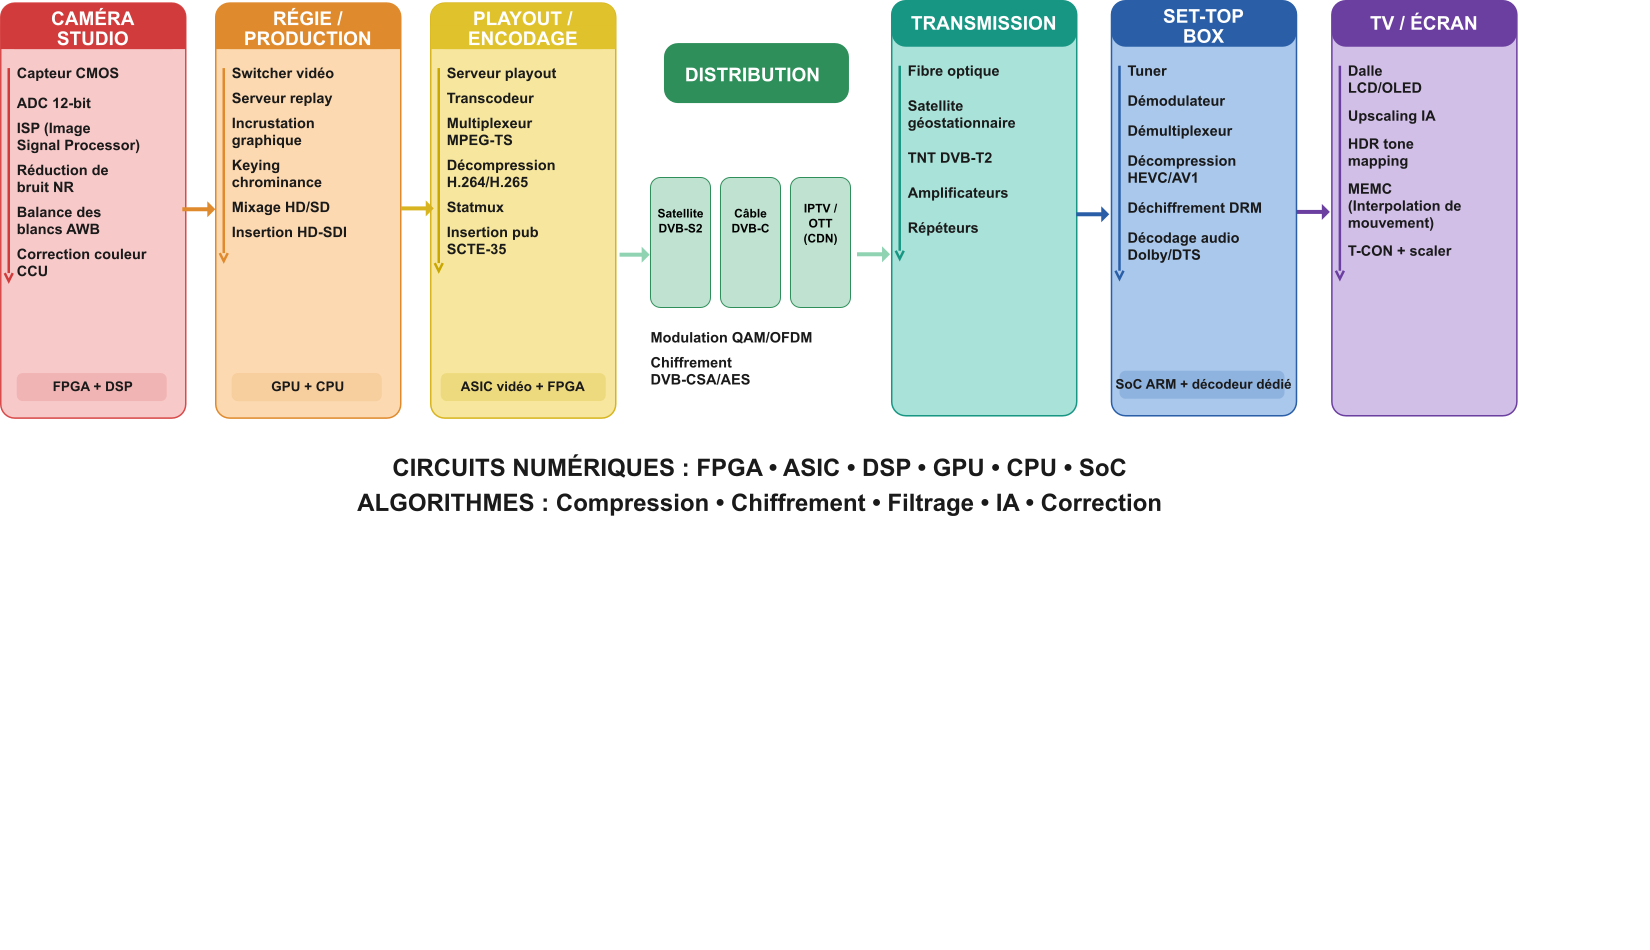
\includegraphics[width=\textwidth]{./images/chaine-diffusion-tv.png}
  \end{center}
\end{frame}
